\section{Computing the 50 Largest Eigenvalues of ATA} \label{sec:50eigen}
Having now found a way to compute an eigenvalue given a matrix, we need a way to calculate the $i$ largest eigenvalues and and associated eigenvectors in order to perform ISVD. To do this, we can use the fact that every eigenvector in a symmetric matrix, for example $\mtrA^T\mtrA$, must be orthogonal to every other eigenvector. Thus, we can modify our algorithm for finding an eigenvalue from Section \ref{sec:firstEigen}
to ensure that the vector that we are currently constructing is orthogonal to every eigenvector we
have already constructed. In other words, if we are in the midst of computing eigenvector $\mvec{V}_i \approx \mvec{u}_n$ then we want to ensure that $\mvec{u}_{n+1}^{T}\mvec{V}_1=\mvec{u}_{n+1}^{T}\mvec{V}_2=\mvec{u}_{n+1}^{T}\mvec{V}_{i-1}=0$.

To do this, we can utilize  \textit{Gram-Schmidt Orthogonalization}. Specifically, from
a next guess vector $\mvec{u}_{n+1}^{*} =\ \mtrA^T\mtrA\mvec{u}_{n}$ having previously computed 
$r$ eigenvectors $\mvec{V}_1 \dots \mvec{V}_r$, we can "orthogonalize" the vector by computing:
\begin{equation*}
    \mvec{u}_{n+1} = \mvec{u}_{n+1}^{*}-\sum _{j=1}^{r-1}\left(\mvec{u}_{n+1}^{* T\:}\mvec{V_j}\right)\mvec{V_j}
\end{equation*}

Relying on these ideas, we can now alter our algorithm from Section \ref{sec:firstEigen} to compute the $i=50$ largest eigenvalues and associated eigenvectors of $\mtrA^T\mtrA$. This creates the following algorithm to assign the eigenvectors to the
matrix $\mtrV$:
\begin{enumerate}
    \item  Initialize $\mvec{V}_1$ to $\mvec{V}_{50}$ as a matrix of zeroes (in this case of the Mariana Trench, this matrix will have size $1440 \times 50$))
    \item for $i=1$ to $50$
    \begin{enumerate}
    \item $\mvec{u}_1 = $  a random unit vector with the correct number of components.
    \item $\mvec{u}_{n+1}^{*} :=\ \mtrA^T\mtrA\mvec{u}_{n} $
    \item $\mvec{u}_{n+1} := \mvec{u}_{n+1}^{*}-\sum _{j=1}^{i-1}\left(\mvec{u}_{n+1}^{* T\:}\mvec{V_j}\right)\mvec{V_j}$
    \item $\mvec{u}_{n+1} := \frac{\mvec{u}_{n+1}}{\lVert\mvec{u}_{n+1}\rVert}$
    \item Repeat b-d until $\lVert \mvec{u}_{n+1} -  \mvec{u}_{n} \rVert < \text{acceptable precision}$
    \item Store the final $\mvec{u}_{n+1}$ as $\mvec{V}_i$
    \end{enumerate}
\end{enumerate}
Converting this algorithm into Matlab, we are now able to compute the $50$ largest eigenvalues, via their eigenvectors, of $\mtrA^T\mtrA$. Again, $\mtrA$ represents the depth data for the Mariana Trench. See Section \ref{sec:codeWithOutput} for the code used for the calculation. Having calculated these eigenvalues, with the corresponding eigenvectors stored as $\mtrV$, we can now create a semilog plot of them, as shown in \autoref{fig:50EVect}.
\begin{figure}[H]
    \centering
    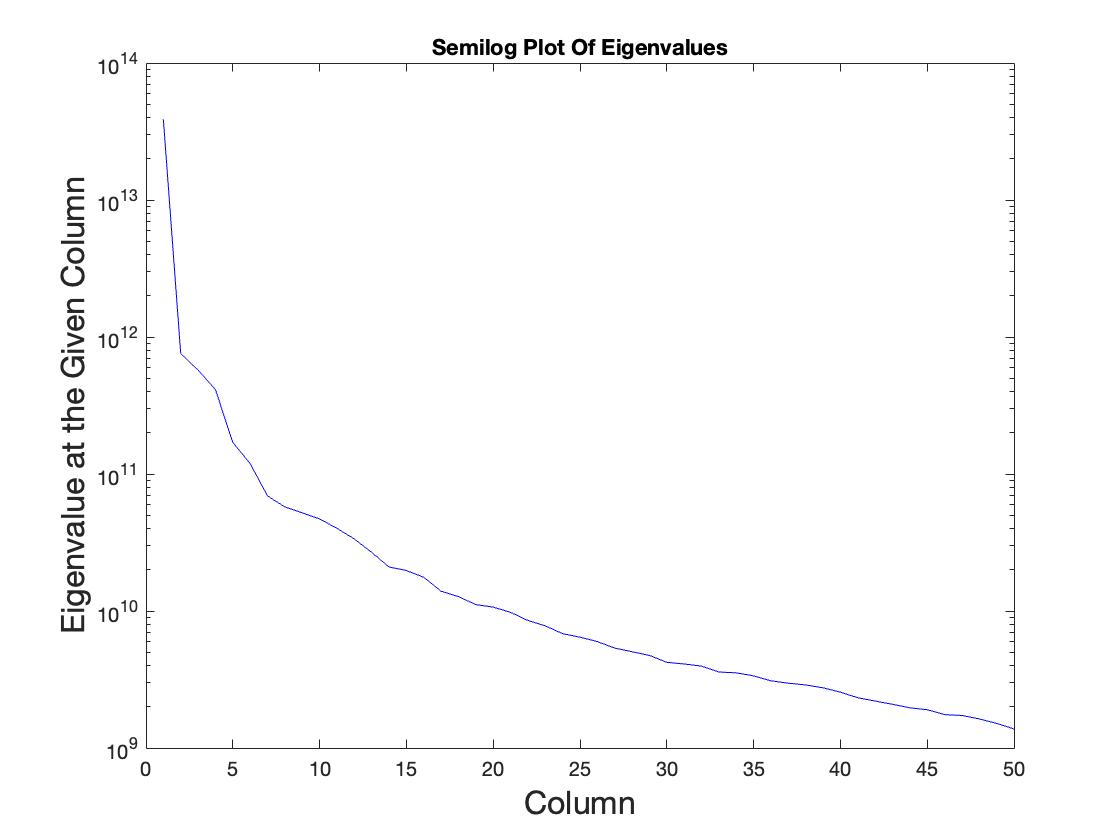
\includegraphics[width=0.6\textwidth]{./imgs/EigenvaluesFor50.jpg}
    \caption{Semilog Plot of the 50 Largest Eigenvalues of $\mtrA^T\mtrA$ \\ Note: Eigenvalues from Columns of $\mtrV$}
    \label{fig:50EVect}
\end{figure}
